\documentclass{article}
\usepackage[utf8]{inputenc}
\usepackage[russian]{babel}
\usepackage{listings}
\usepackage[a4paper, total={6in, 10in}]{geometry}
\usepackage{graphicx}
\usepackage{float}
\usepackage{wrapfig}

\title{Документация к построению ER и реляционных диаграмм}
\author{Григорьев Роман, Бермишев Владислав}

\begin{document}

\maketitle

\newpage
\tableofcontents

\newpage

\section{Описание грамматики}
\subsection{Грамматика}
\qquad Программа представляет ER-диаграмму и реляционную диаграмму по грамматике, приведённой ниже:
\begin{lstlisting}
Grammar ::= Rule+

Rule ::= Entity_definition | Relation_definition | type_sybtype_relation_definition

Entity_definition ::= [Name] -> eps; 
([Name].attr = [List], [Name].ident = [List]) | ([Name].ident = [List], 
[Name].attr = [List])

[Name] ::= ([A-z]|[0-9])*

[List] ::= (([Name],)*[Name])

Relation_definition := [Name]'1 -> [Name]'2; 
[Name]'1.cardinality = [Cardinality], 
[Name]'2.cardinality = [Cardinality], 
([Name]'1.ident ::= [Name]'2.ident | [Name]'2.ident ::= [Name]'1.ident | eps)

[Cardinality] = (0|1|N)-(0|1|N)

[type_subtype_definition] := [Name]'1 -> ([Name]'i |)*[Name]'n; 
([Name]'i.attr = [List])^n, 
[Name]'1.subtypes = [inclusive | exclusive]
\end{lstlisting}

\subsection{Дополнительные условия на грамматику}
\justifying

\flushleft

\begin{itemize}
\item \verb|Entity_definition| для конкретного [Name] не может встречаться больше 1 раза.
\item Не более 1 определения attr и ident в \verb|Entity_definition|.
\item Нельзя определять attr и ident другого Entity отличного от определённого в \verb|Entity_definiton|.
\item Обязательность задания 2 пар чисел кардинальности относящимся к этому Relation в \verb|Relation_definition|.
\item Не более 1 зависимости идентификаторов (Name]'1.ident ::= [Name]'2.ident) в \verb|Relation_definition|.
\item Обязательность определения [Name]'1 и [Name]'2 до определения отношения.
\tem  При указаний зависимости идентификаторов, обязательность непустого пересечения идентификаторов [Name]'1 и [Name]'2.
\item Не более 1 определения аттрибутов в \verb|type_subtype_template| для [Name]'i.
\item Обязательность определения сущности [Name]'1 до определения \verb|type_sybtype_template|.
\item Не более 1 определния типа связи шаблона ([Name]'1.subtypes = ...), значение по умолчанию будет inclusive.
\end{itemize}




\section{Построение диаграмм}
\subsection{Возможности}
\qquad Данная программа позволяет строить ER-диаграмму грамматики и преобразовывать её в реляционную. Диаграммы представляются в виде файлов с расширением .svg.


\qquad Также есть возможность автоматического извлечения таблицы кардинальностей из описания модели. Данная таблица представляется в виде файла с расширением .csv.


\subsection{Установка и запуск}
\qquad Для запуска программы вам понадобится язык программирования C++. Далее склонируйте репозиторий и установите библиотеку для автоматической визуализации диаграмм:

\begin{lstlisting}
git clone https://github.com/VladBermishev/FormalLanguageTheory_Labs/lab5
cd lab5
sudo apt-get install libgraphviz-dev
\end{lstlisting}

\qquad Для работы программы необходимо создать конфигурационный файл и указать в нем параметры модели. Для запуска программы требуется собрать проект:

\begin{lstlisting}
mkdir build ; cd build
cmake ../ -DBUILD=Release
cmake --build . --target lab5 -j 3
\end{lstlisting}

\qquad Пример запуска программы:
\begin{lstlisting}
./lab5 < tests/1
or
./lab5 tests/1
\end{lstlisting}

\qquad Программа выведет ER-модель, реляционную и таблицу кардинольностей для нашей модели.

\subsection{Структура проекта}

\begin{lstlisting}
FormalLanguageTheory_Labs/lab5/
- include/lab5/
│   -attribure.h
│   -entity.h
│   -entity_relationship_diagram.h
│   -relation.h
- tests/
│   - 1
- CMakeLists.txt
- main.cpp
- readme.md
\end{lstlisting}

\qquad В репозитории в директории \verb|tests| лежат конфигурационные файлы. В директории \verb|include/lab5/|:
\begin{itemize}
\item в модуле \verb|attribute.h| объявлен класс Attribute, описывающий атрибуты и индефекаторы сущности.
\item в модуле \verb|entity.h| объявлен класс Entity, описывающий сущности.
\item в модуле \verb|entity_relationship_diagram.h| объявлен класс EntityRelationshipDiagram, описывающий класс EntityRelationship и RelationDiagram.
\item в модуле \verb|relation.h| объявлен класс Relation, описывающий отношения между сущностями.

\end{itemize}
\qquad В директории \verb|tests/| представлены тесты к данной программе. Основной модуль - \verb|main.cpp|, в нем находится код, использующийся для построения диаграм.

\subsection{Настраиваемые параметры}
\qquad Необязательным параметром является путь до входной грамматики.


\section{Примеры работы}

\qquad Запустим код, используя конфигурационный файл \verb|tests\1|.На вывод мы получаем 3 файла:
\begin{itemize}
\item Таблицу кардинальностей нашей модели. 

\begin{figure}[h]
\centering
\includegraphics[width=0.8\linewidth]{cardinalities.jpg}
\label{fig:mpr}
\end{figure}

\item ER-модель.

\begin{figure}[h]
\centering
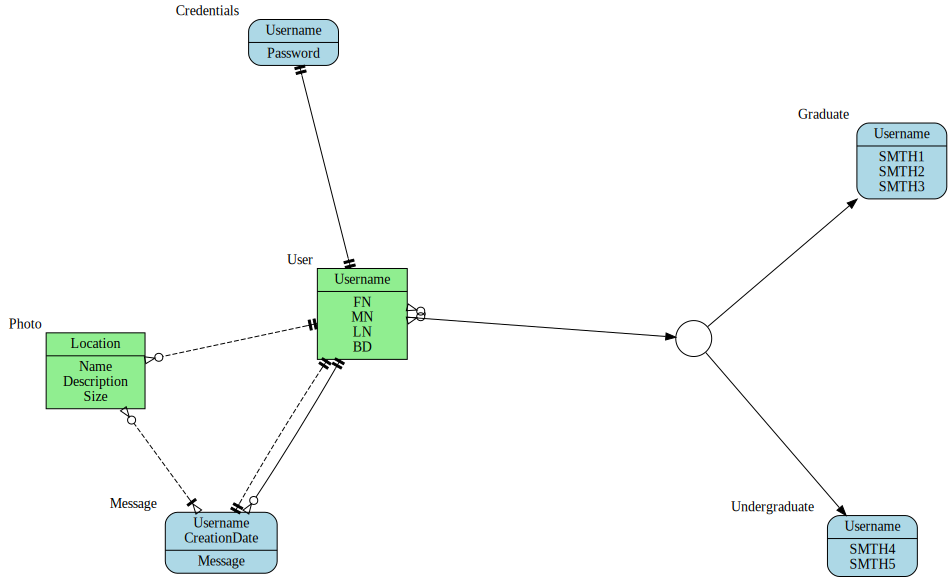
\includegraphics[width=0.8\linewidth]{ER_model.jpg}
\label{fig:mpr}
\end{figure}

\item Реляционную модель.

\begin{figure}[h]
\centering
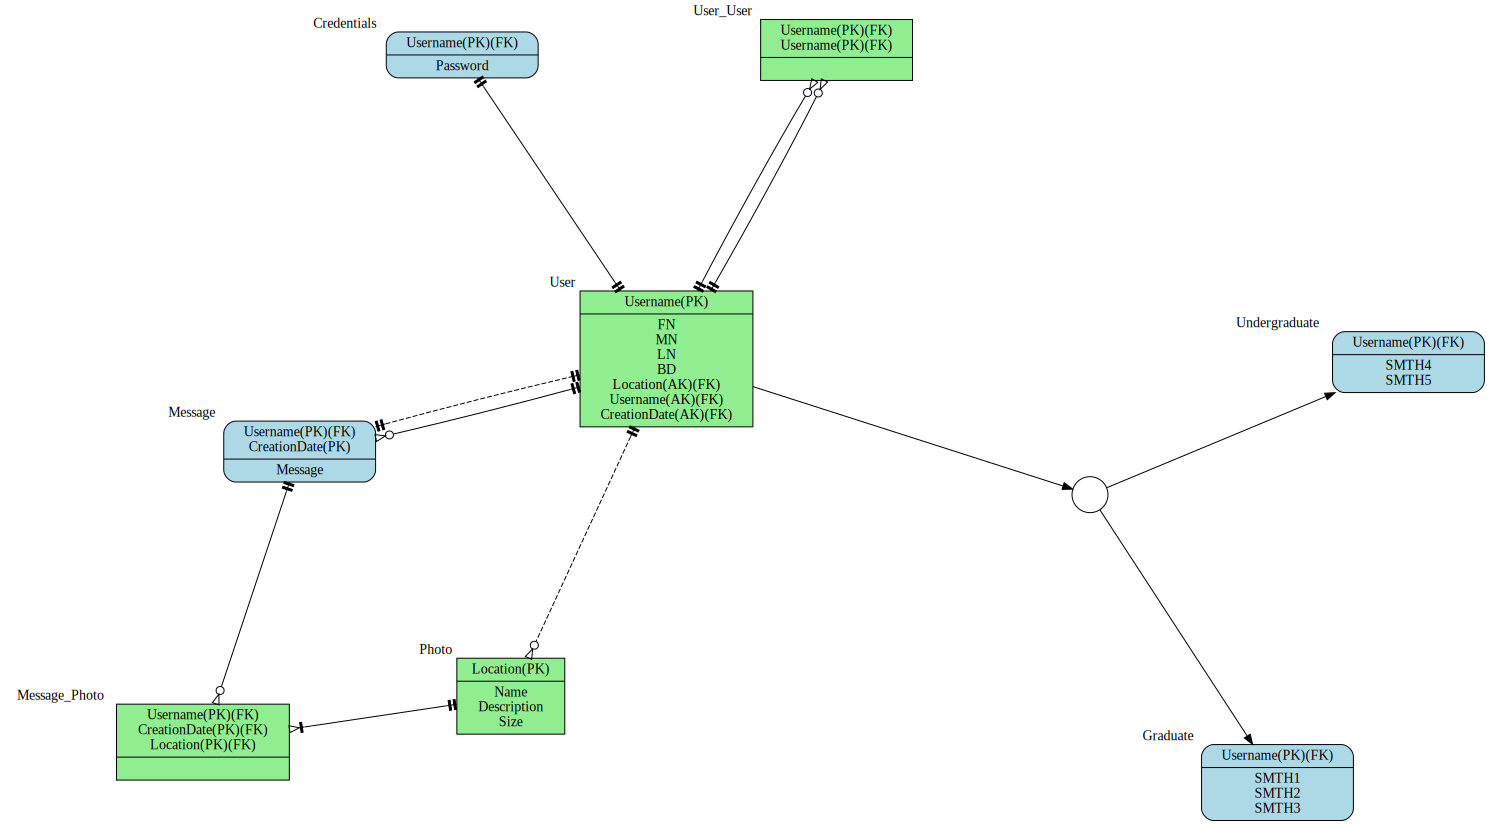
\includegraphics[width=0.8\linewidth]{Relational_model.jpg}
\label{fig:mpr}
\end{figure}

\end{itemize}
\end{document}